\documentclass[12pt]{report}
\usepackage[utf8]{inputenc}
\usepackage[english, russian]{babel}
\usepackage{listings}
\usepackage{graphicx}
\usepackage{float}
\graphicspath{{imgs/}}
\usepackage{amsmath,amsfonts,amssymb,amsthm,mathtools} 
\usepackage{pgfplots}
\usepackage{filecontents}
\usepackage{indentfirst}
\usepackage{eucal}
\usepackage{enumitem}
\frenchspacing

\usepackage{indentfirst} % Красная строка

\usetikzlibrary{datavisualization}
\usetikzlibrary{datavisualization.formats.functions}

\usepackage{amsmath}
\usepackage{fixltx2e}
\usepackage{caption}


\definecolor{bluekeywords}{rgb}{0,0,1}
\definecolor{greencomments}{rgb}{0,0.5,0}
\definecolor{redstrings}{rgb}{0.64,0.08,0.08}
\definecolor{xmlcomments}{rgb}{0.5,0.5,0.5}
\definecolor{types}{rgb}{0.17,0.57,0.68}

\usepackage{listings}
\lstset{language=[Sharp]C,
	captionpos=t,
	numbers=left, %Nummerierung
	numberstyle=\small, % kleine Zeilennummern
	frame=single, % Oberhalb und unterhalb des Listings ist eine Linie
	stepnumber=1,                   
	numbersep=5pt,                
	showspaces=false,
	tabsize=2,
	showtabs=false,
	breaklines=true,
	showstringspaces=false,
	breakatwhitespace=true,
	escapeinside={(*@}{@*)},
	commentstyle=\color{greencomments},
	morekeywords={partial, var, value, get, set},
	keywordstyle=\color{bluekeywords},
	stringstyle=\color{redstrings},
	basicstyle=\ttfamily\small,
}

\usepackage[left=1cm,right=1cm, top=1cm,bottom=2cm,bindingoffset=0cm]{geometry}
% Для измененных титулов глав:
\usepackage{titlesec, blindtext, color} % подключаем нужные пакеты
\definecolor{gray75}{gray}{0.75} % определяем цвет
\newcommand{\hsp}{\hspace{20pt}} % длина линии в 20pt
% titleformat определяет стиль
\titleformat{\chapter}[hang]{\Huge\bfseries}{\thechapter\hsp\textcolor{gray75}{|}\hsp}{0pt}{\Huge\bfseries}

\usepackage{array}
\newcommand{\head}[2]{\multicolumn{1}{>{\centering\arraybackslash}p{#1}}{#2}}

% plot
\usepackage{pgfplots}
\usepackage{filecontents}
\usetikzlibrary{datavisualization}
\usetikzlibrary{datavisualization.formats.functions}

\begin{document}
	%\def\chaptername{} % убирает "Глава"
	\thispagestyle{empty}
	\begin{titlepage}
		\noindent \begin{minipage}{0.15\textwidth}
			
\includegraphics[width=\linewidth]{b_logo}
		\end{minipage}
		\noindent\begin{minipage}{0.9\textwidth}\centering
			\textbf{Министерство науки и высшего образования Российской Федерации}\\
			\textbf{Федеральное государственное бюджетное образовательное учреждение высшего образования}\\
			\textbf{~~~«Московский государственный технический университет имени Н.Э.~Баумана}\\
			\textbf{(национальный исследовательский университет)»}\\
			\textbf{(МГТУ им. Н.Э.~Баумана)}
		\end{minipage}
		
		\noindent\rule{18cm}{3pt}
		\newline\newline
		\noindent ФАКУЛЬТЕТ $\underline{\text{«Информатика и системы управления»}}$ \newline\newline
		\noindent КАФЕДРА $\underline{\text{«Программное обеспечение ЭВМ и информационные технологии»}}$\newline\newline\newline\newline\newline\newline\newline\newline\newline\newline\newline
		
		
		\begin{center}
			\noindent\begin{minipage}{1.3\textwidth}\centering
				\Large\textbf{  Отчет по лабораторной работе №15-16}\newline
				\textbf{по дисциплине \newline "Функциональное и логическое программирование"}\newline\newline
			\end{minipage}
		\end{center}
		
		\noindent\textbf{Тема} $\underline{\text{Формирование эффективных программ и рекурсия на Prolog}}$\newline\newline
		\noindent\textbf{Студент} $\underline{\text{Малышев И. А.}}$\newline\newline
		\noindent\textbf{Группа} $\underline{\text{ИУ7-61Б}}$\newline\newline
		\noindent\textbf{Оценка (баллы)} $\underline{\text{~~~~~~~~~~~~~~~~~~~~~~~~~~~}}$\newline\newline
		\noindent\textbf{Преподаватель: } $\underline{\text{Толпинская Н. Б.}}$\newline\newline\newline
		
		\begin{center}
			\vfill
			Москва~---~\the\year
			~г.
		\end{center}
	\end{titlepage}
	
	
	\setcounter{page}{2}

\chapter*{Лабораторная работа №15}
\section*{Задание}

В одной программе написать правила, позволяющие найти:

\begin{enumerate}
	\item Максимум из двух чисел:
	\begin{itemize}
		\item Без использования отсечения;
		\item С использованием отсечения;
	\end{itemize}
	\item Максимум из трех чисел:
	\begin{itemize}
		\item Без использования отсечения;
		\item С использованием отсечения.
	\end{itemize}
\end{enumerate}

Убедиться в правильности результатов. Для каждого случая из пункта 2 обосновать необходимость всех условий тела. Для одного из вариантов ВОПРОСА и каждого варианта задания 2 составить таблицу, отражающую конкретный порядок работы системы.

Так как резольвента хранится в виде стека, то состояние резольвенты требуется отображать в столбик: вершина – сверху! Новый шаг надо начинать с нового состояния резольвенты!


\newpage
\section*{Решение}

\begin{lstlisting}
domains
	num = integer

predicates
	max2(num, num, num)
	max3(num, num, num, num)
	
	max2clipping(num, num, num)
	max3clipping(num, num, num, num)

clauses
	max2(N1, N2, N2) :- N2 >= N1.
	max2(N1, N2, N1) :- N1 >= N2.
	
	max3(N1, N2, N3, N3) :- N3 >= N1, N3 >= N2.
	max3(N1, N2, N3, N2) :- N2 >= N1, N2 >= N3.
	max3(N1, N2, N3, N1) :- N1 >= N2, N1 >= N3.
	
	max2clipping(N1, N2, N2) :- N2 >= N1, !.
	max2clipping(N1, _, N1).
	
	max3clipping(N1, N2, N3, N3) :- N3 >= N2, N3 >= N1, !.
	max3clipping(N1, N2, _, N1) :- N1 >= N2, !.
	max3clipping(_, N2, _, N2).

goal
	max2(1, 4, Max).
	max2clipping(1, 4, Max).
	max3(133, 4, 5, Max).
	max3clipping(133, 4, 5, Max).
\end{lstlisting}

\section*{Порядок работы}

\begin{figure}[H]
	\begin{center}
		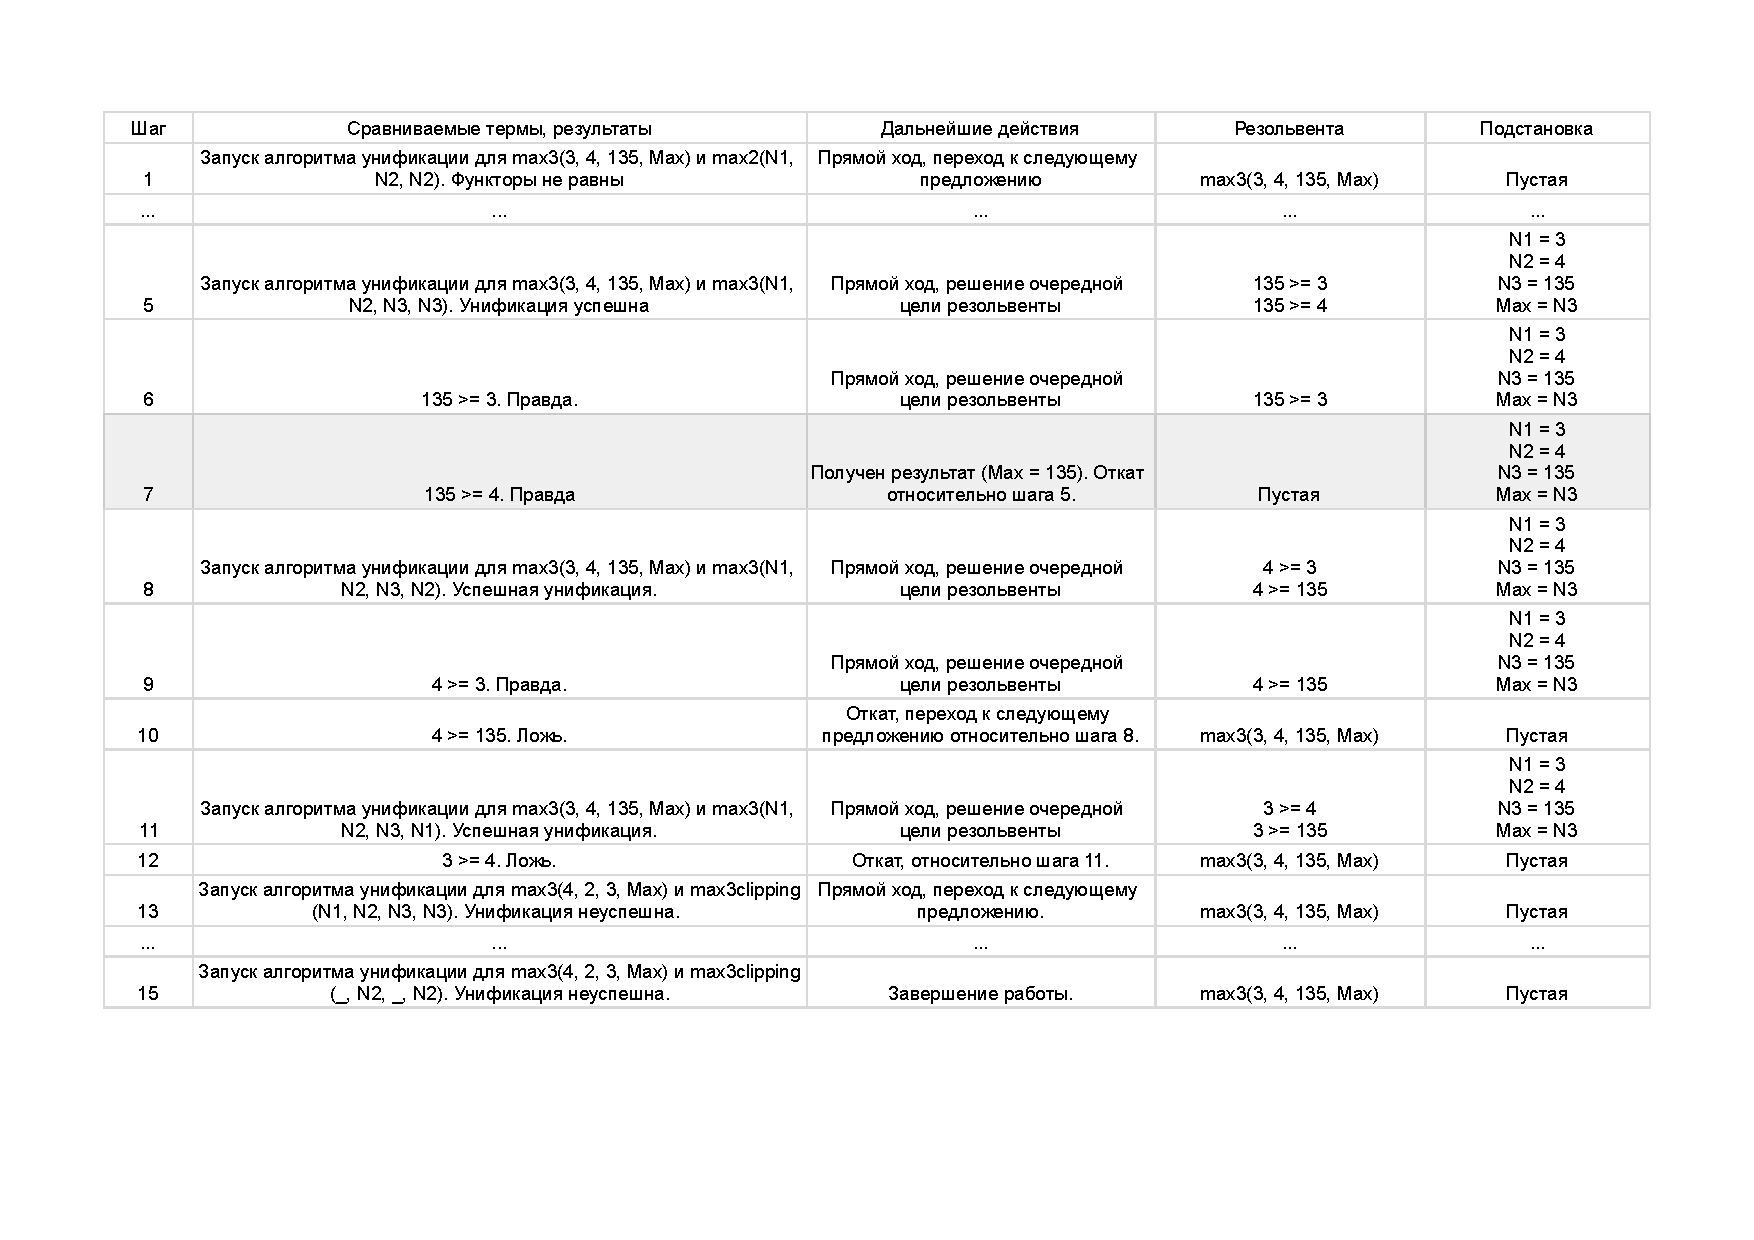
\includegraphics[scale=0.7]{imgs/table_15_01.pdf}
	\end{center}
\end{figure}

\begin{figure}[H]
	\begin{center}
		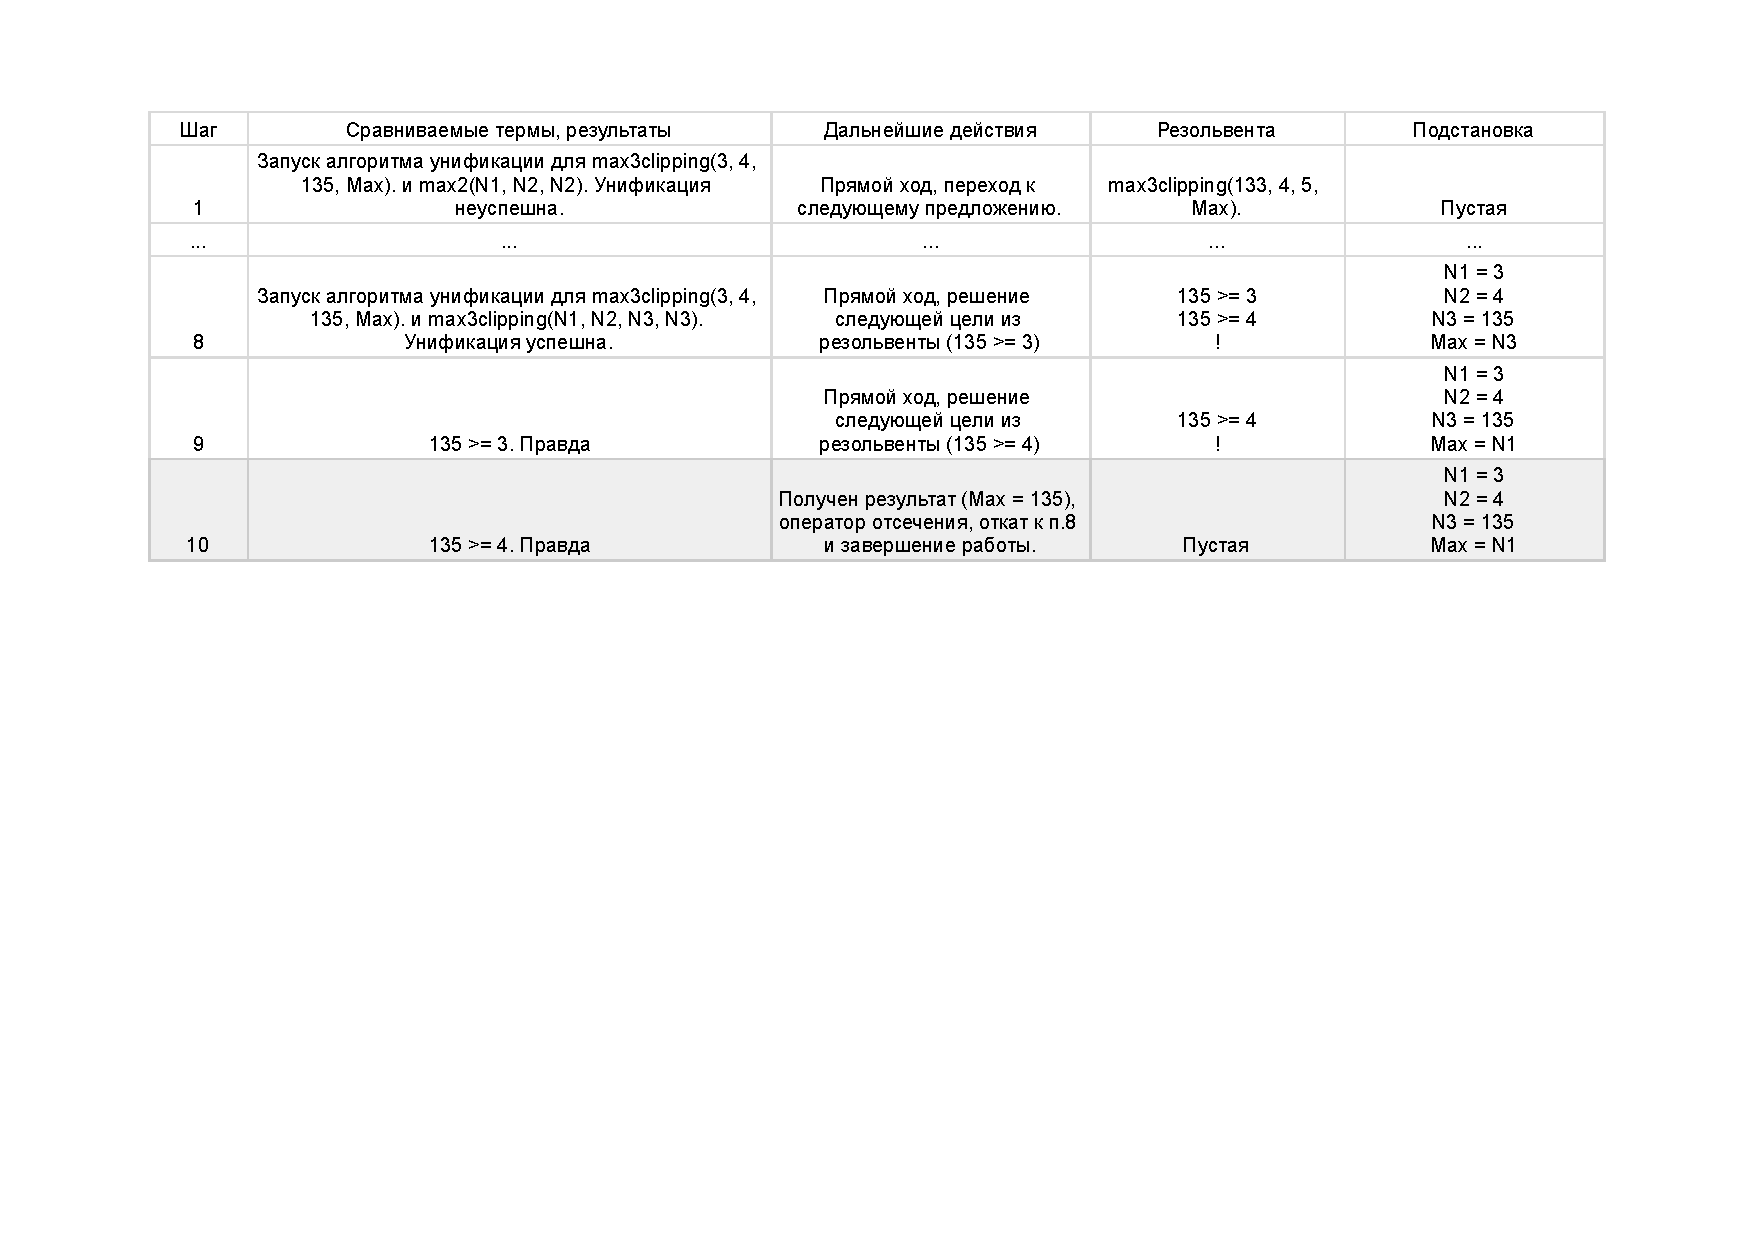
\includegraphics[scale=0.7]{imgs/table_15_02.pdf}
	\end{center}
\end{figure}

\chapter*{Лабораторная работа №16}

\section*{Постановка задачи}

Используя хвостовую рекурсию, разработать программу, позволяющую найти:

\begin{enumerate}
	\item n!;
	\item n-e число Фибоначчи.
\end{enumerate}

Для одного из вариантов ВОПРОСА и каждого задания составить таблицу,
отражающую конкретный порядок работы системы:

Т.к. резольвента хранится в виде стека, то состояние резольвенты требуется отображать
в столбик: вершина – сверху! Новый шаг надо начинать с нового состояния резольвенты!

\newpage
\section*{Решение}

\begin{lstlisting}
domains
	num = integer

predicates
	fact(num, num)
	rec_fact(num, num, num)
	
	fib(num, num)
	rec_fib(num, num, num, num)

clauses
	rec_fact(N, Res, Acc) :- N > 1, !, NewN = N - 1, NewAcc = Acc * N, rec_fact(NewN, Res, NewAcc).
	rec_fact(_, Res, Acc) :- Res = Acc.
	fact(N, Res) :- rec_fact(N, Res, 1).
	
	rec_fib(N, F1, F2, Res) :- N > 2, !, NewF1 = F2, NewF2 = F1 + F2, NewN = N - 1, rec_fib(NewN, NewF1, NewF2, Res).
	rec_fib(_, _, B, Res) :- Res = B.
	fib(N, Res) :- rec_fib(N, 1, 1, Res).

goal
	fact(4, Res).
	fib(7, Res).
\end{lstlisting}

\section*{Порядок работы}

\begin{figure}[H]
	\begin{center}
		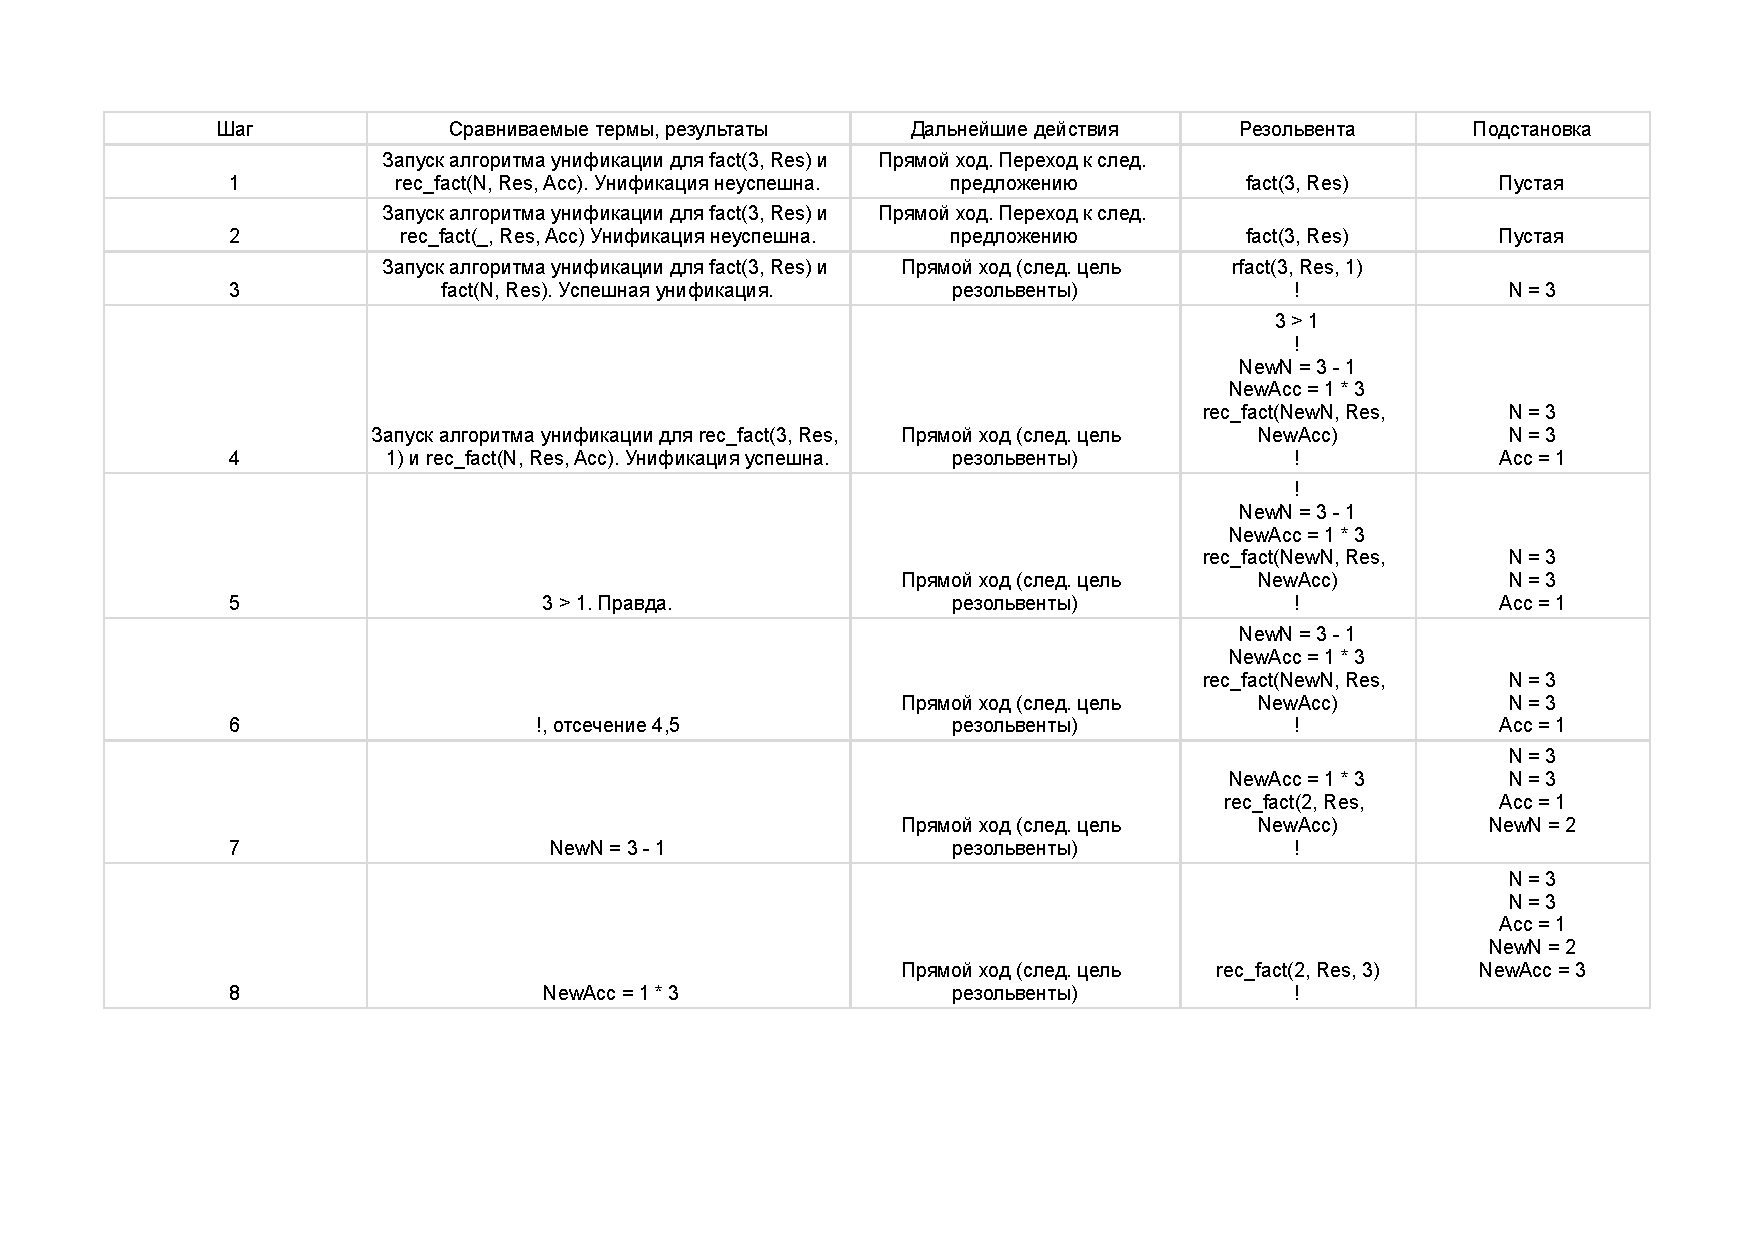
\includegraphics[scale=0.7]{imgs/table_16_01-1.pdf}
	\end{center}
\end{figure}

\begin{figure}[H]
	\begin{center}
		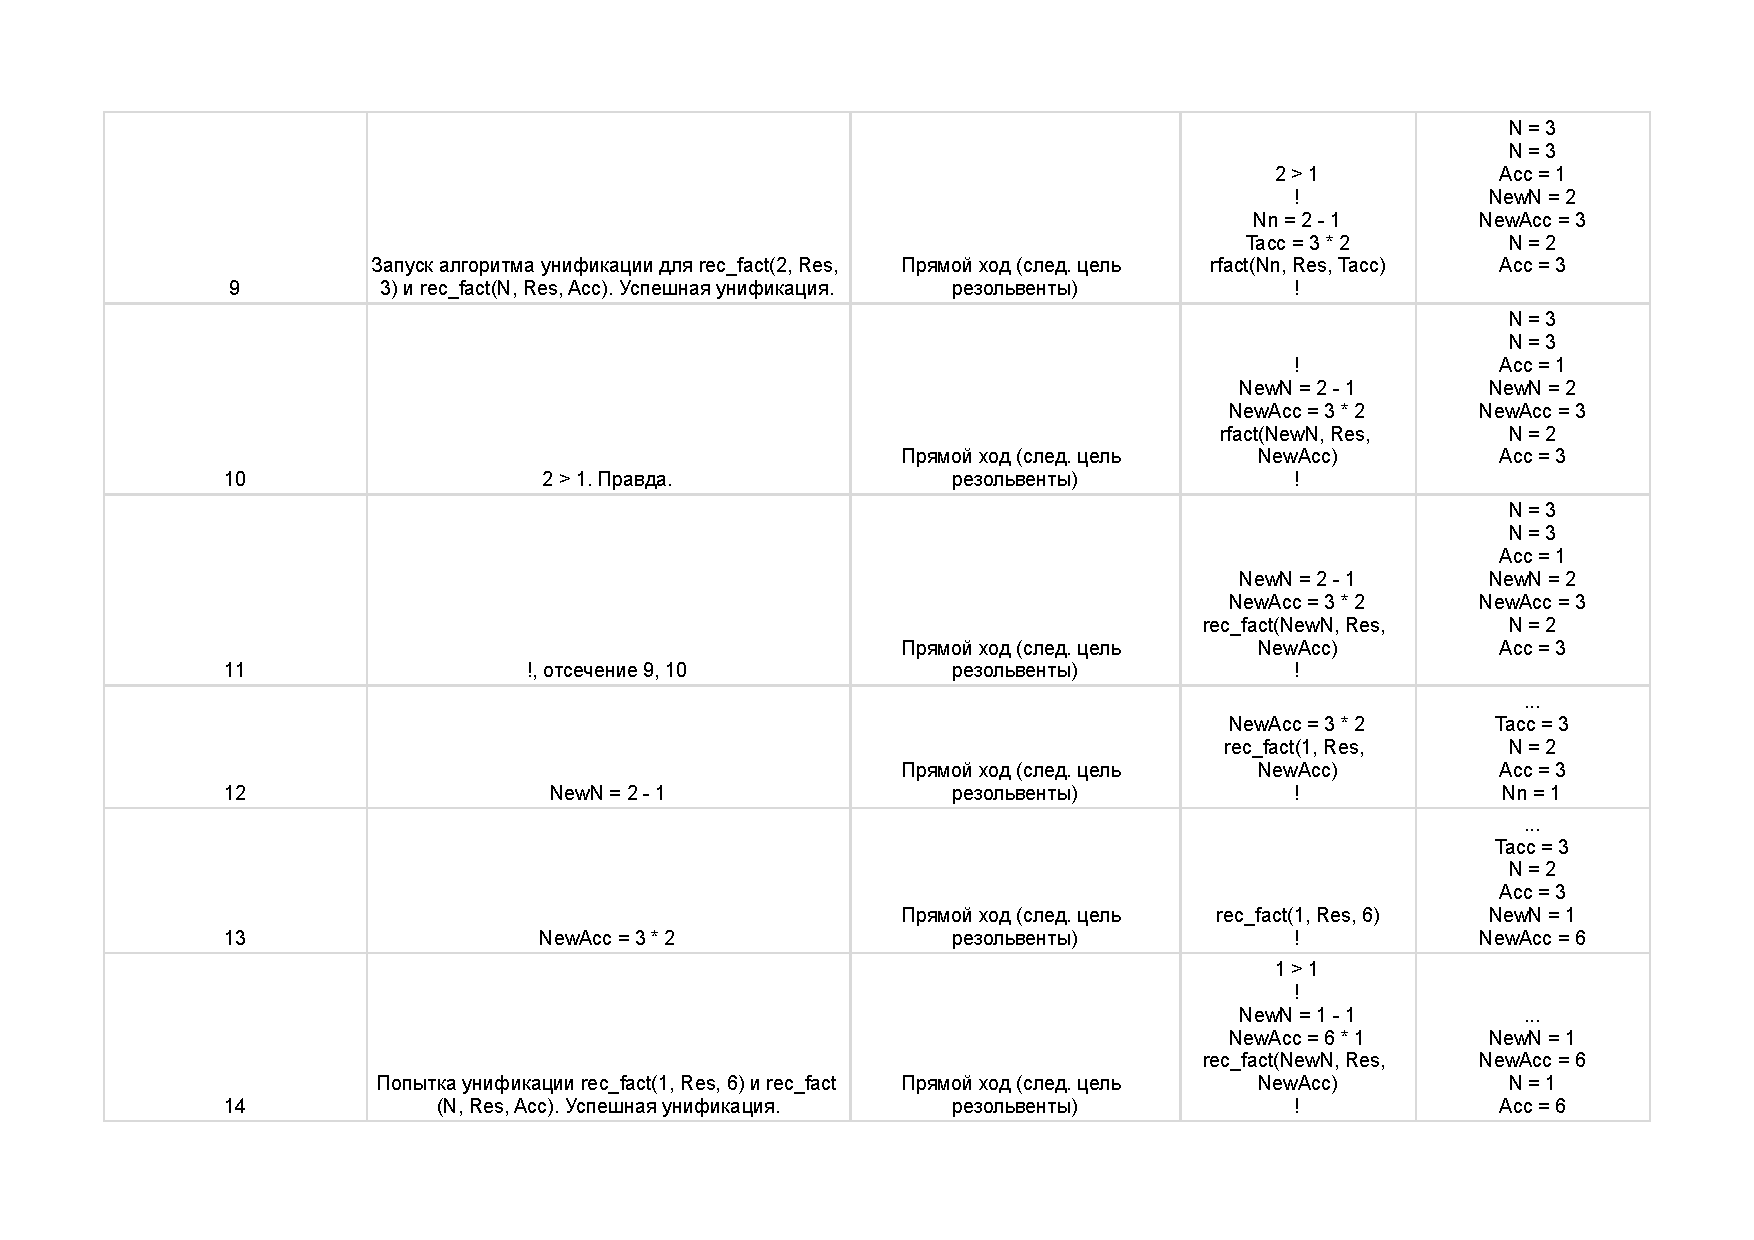
\includegraphics[scale=0.7]{imgs/table_16_01-2.pdf}
	\end{center}
\end{figure}

\begin{figure}[H]
	\begin{center}
		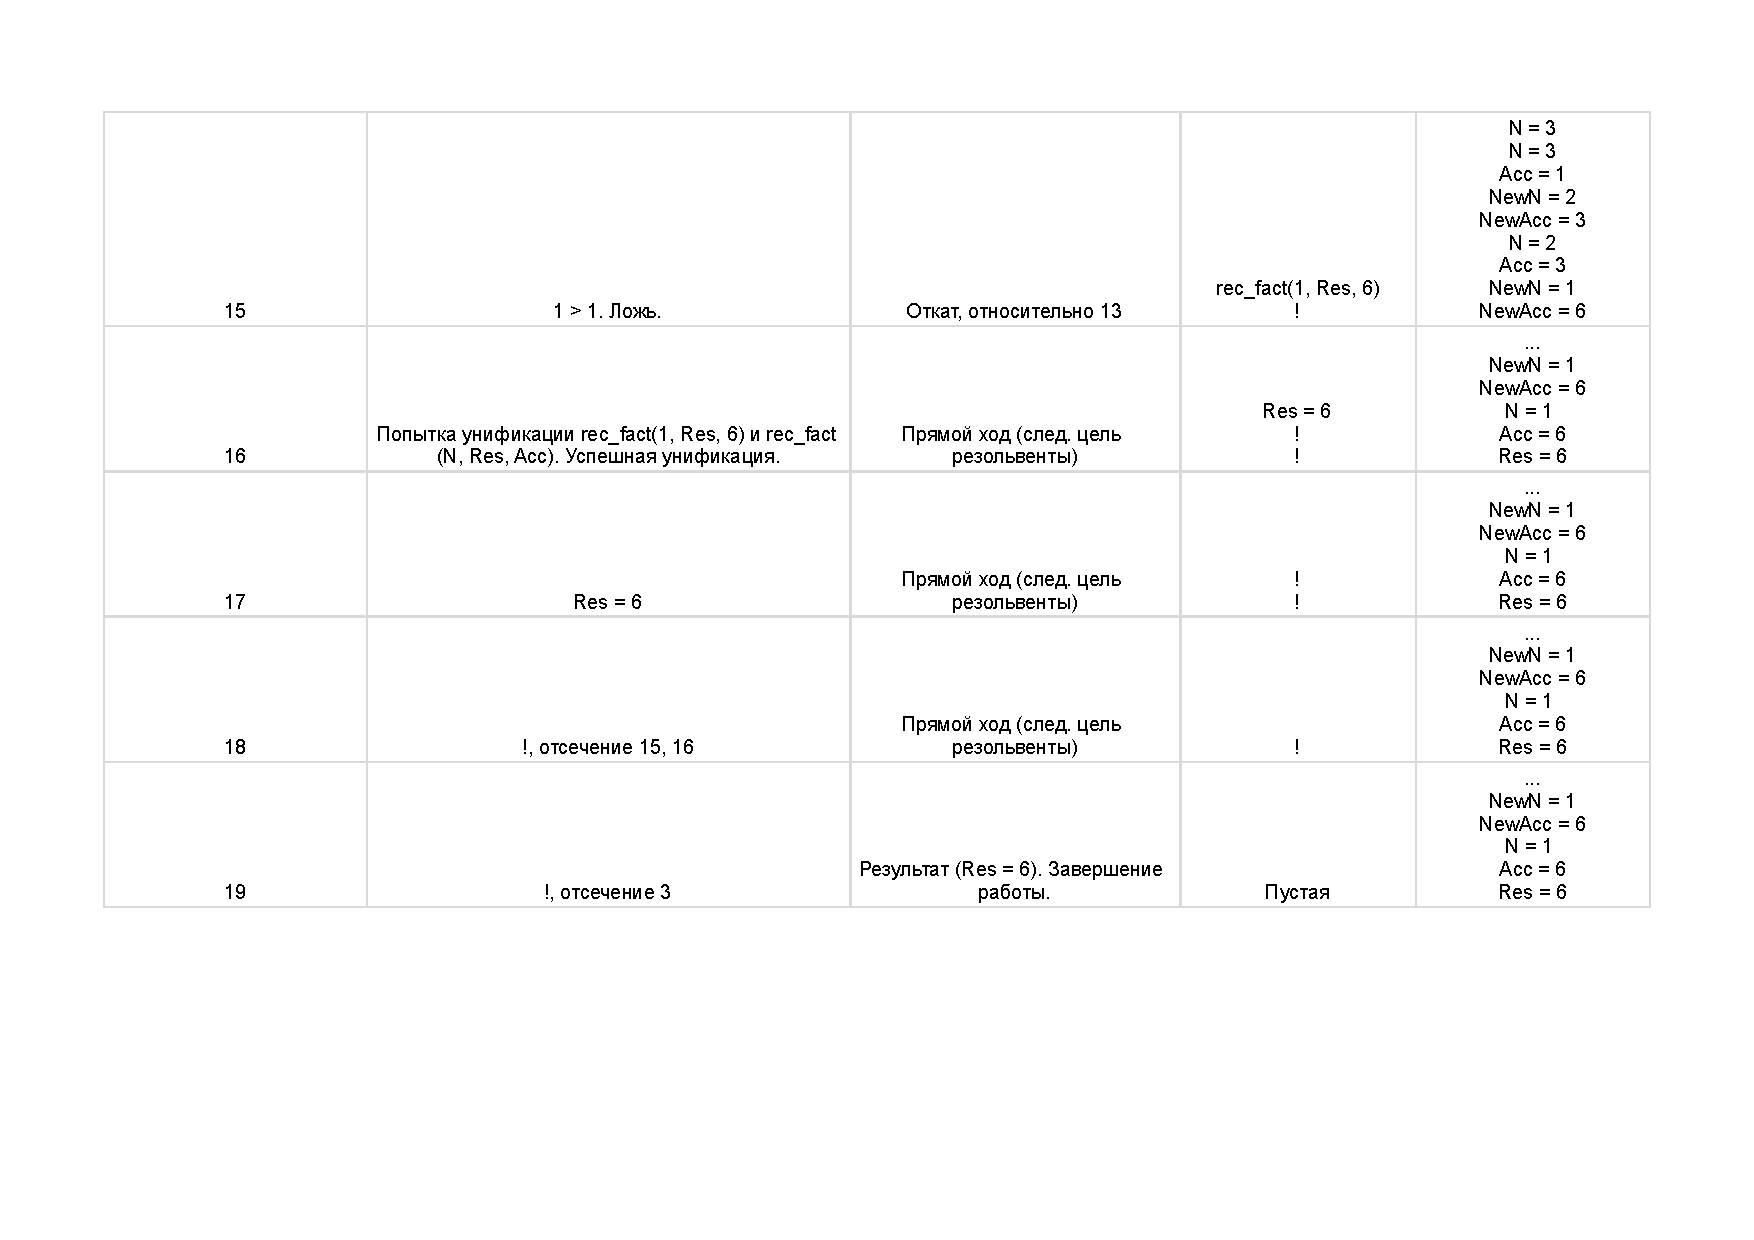
\includegraphics[scale=0.7]{imgs/table_16_01-3.pdf}
	\end{center}
\end{figure}


\begin{figure}[H]
	\begin{center}
		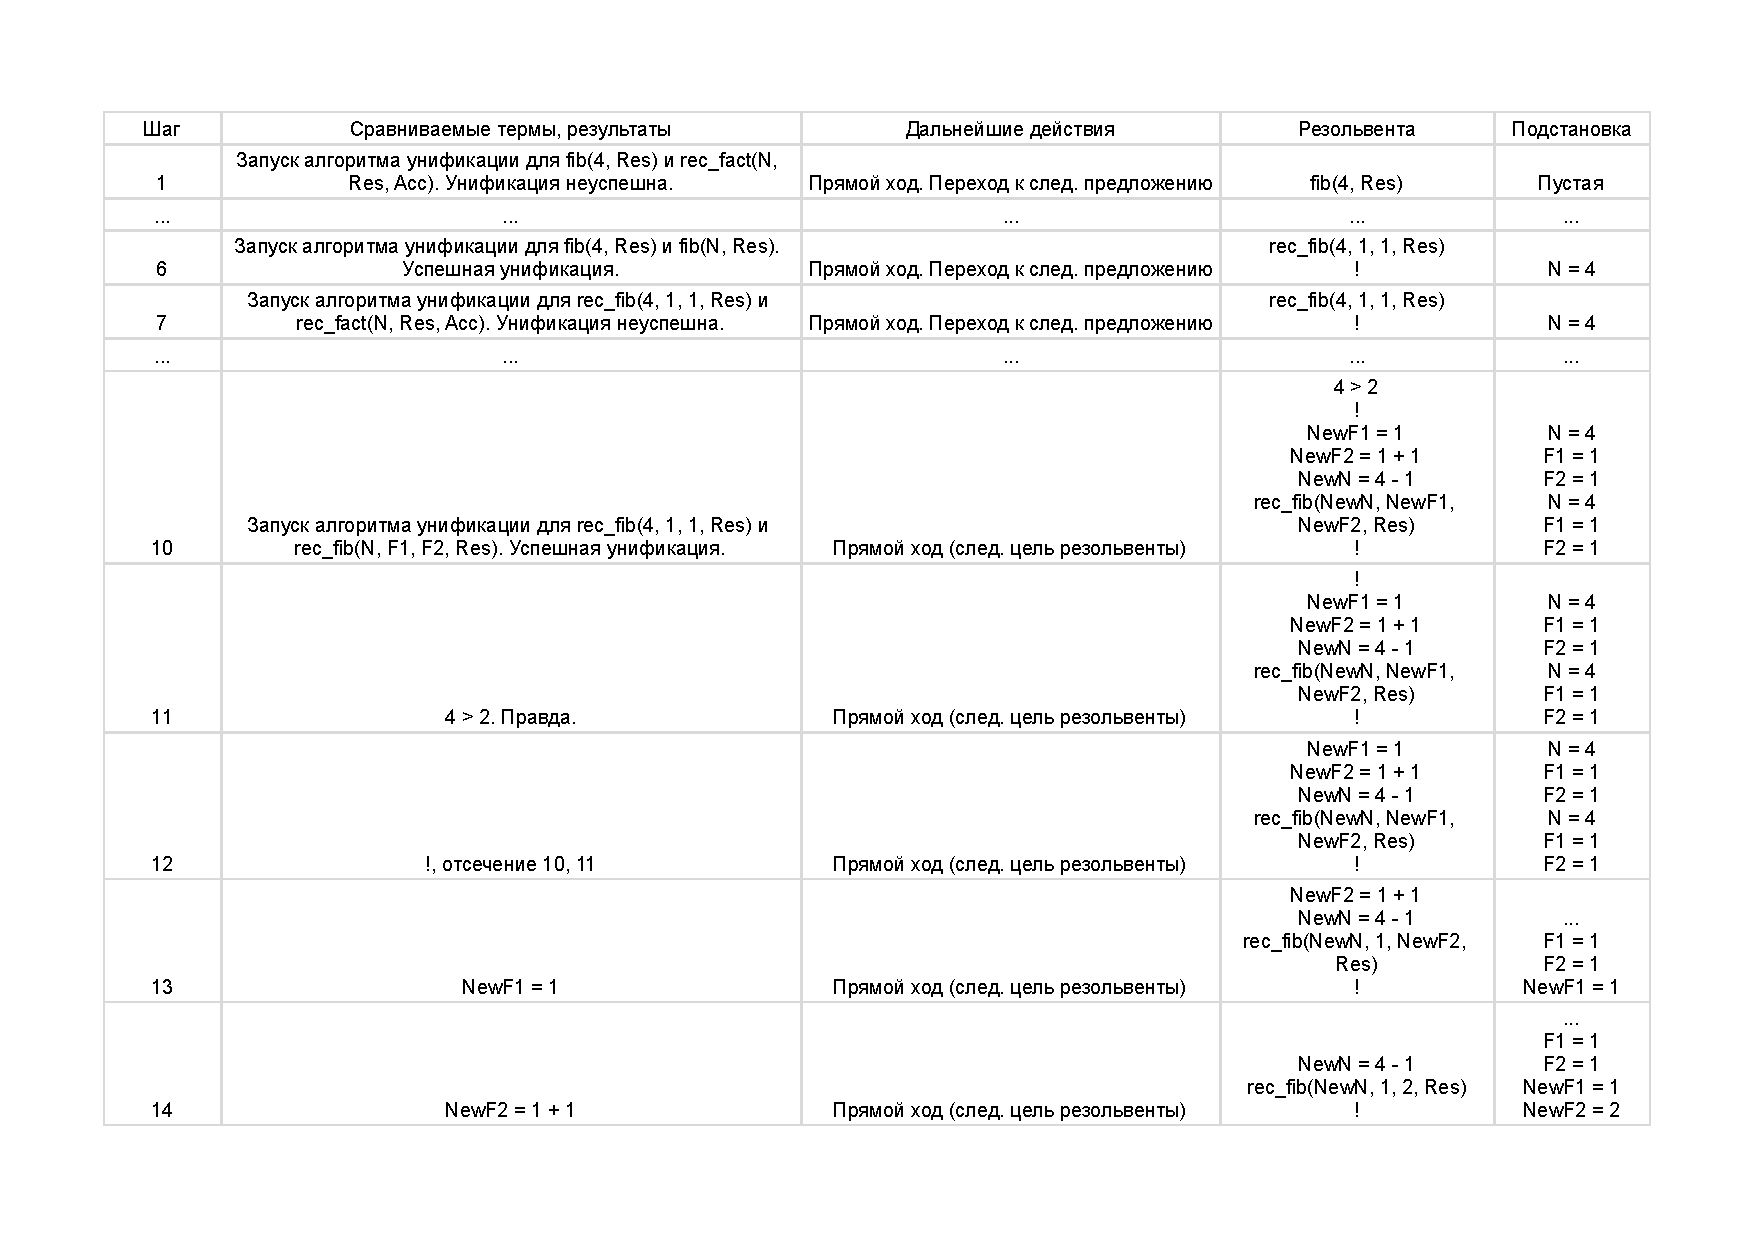
\includegraphics[scale=0.7]{imgs/table_16_02-1.pdf}
	\end{center}
\end{figure}

\begin{figure}[H]
	\begin{center}
		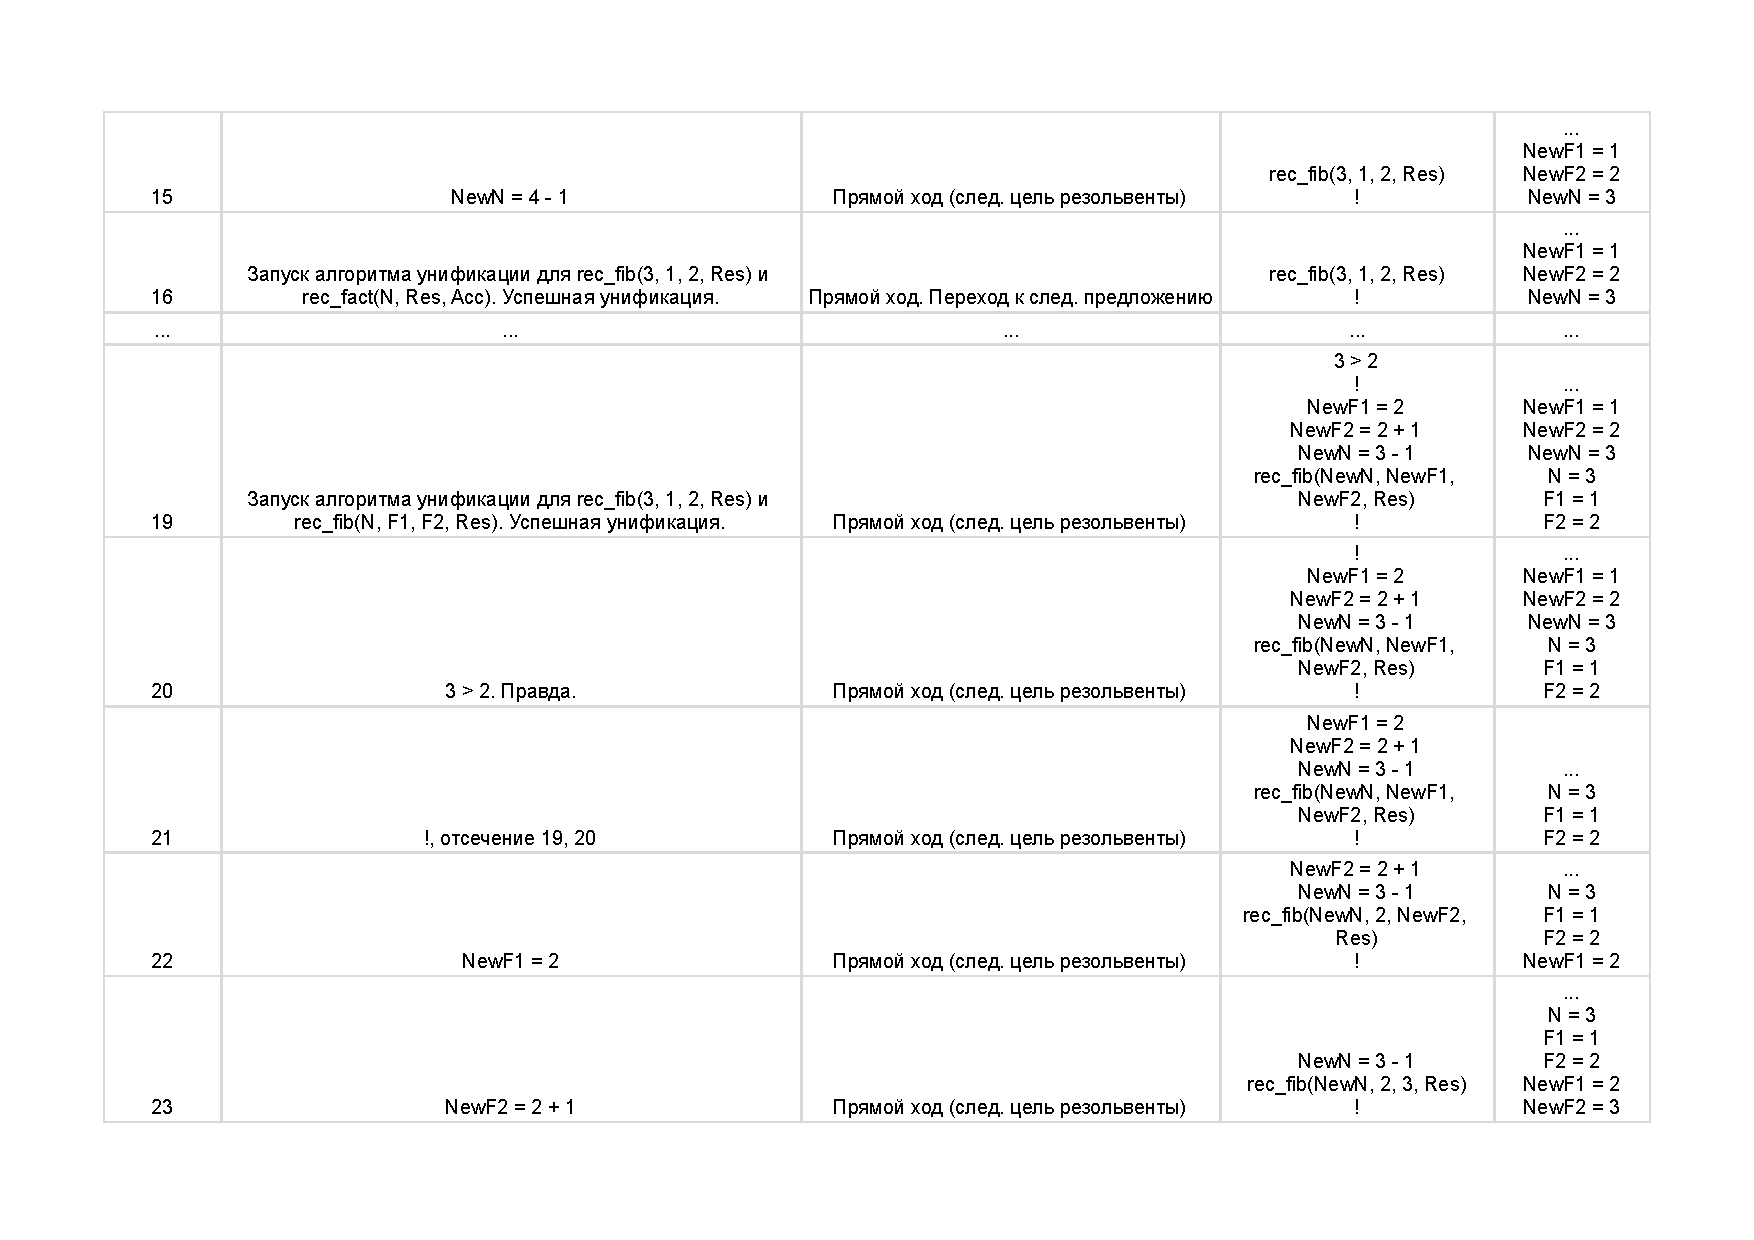
\includegraphics[scale=0.7]{imgs/table_16_02-2.pdf}
	\end{center}
\end{figure}

\begin{figure}[H]
	\begin{center}
		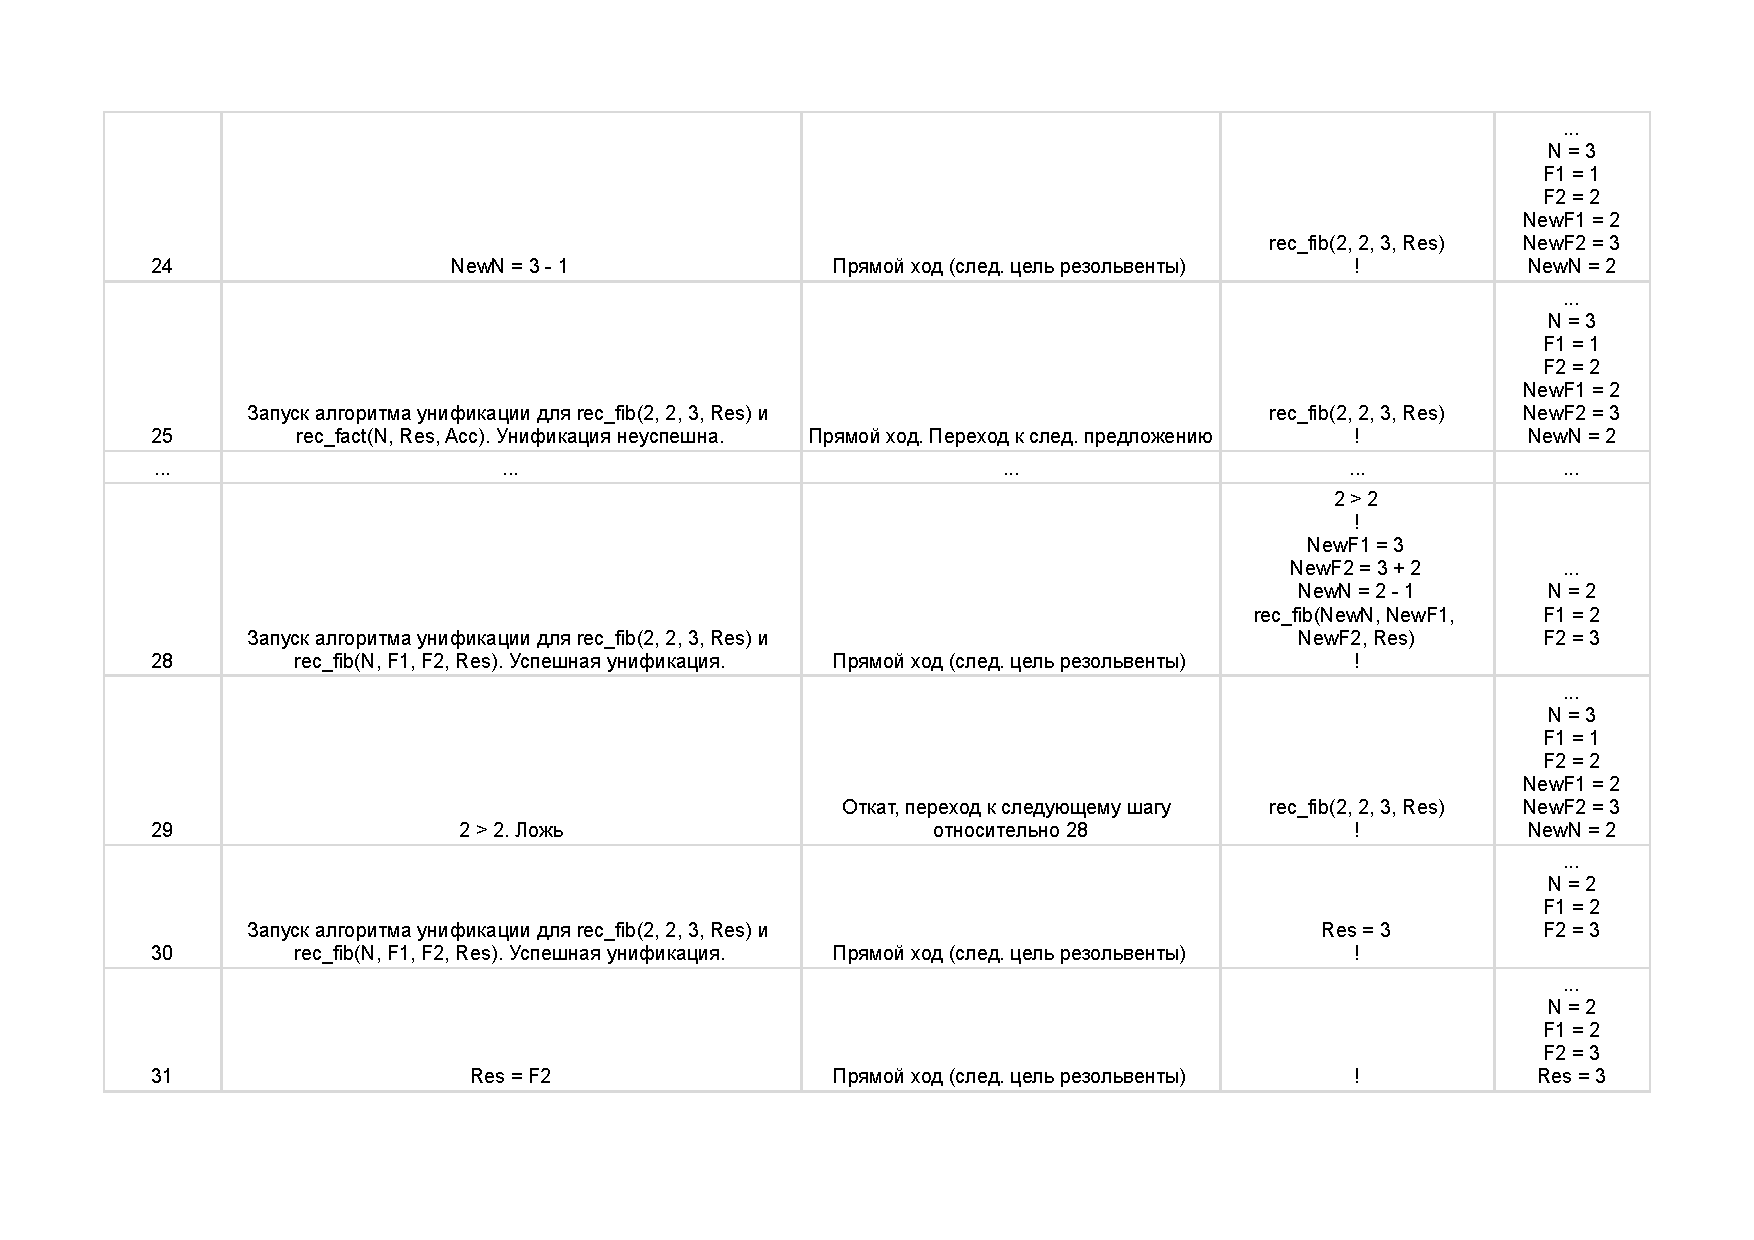
\includegraphics[scale=0.7]{imgs/table_16_02-3.pdf}
	\end{center}
\end{figure}

\begin{figure}[H]
	\begin{center}
		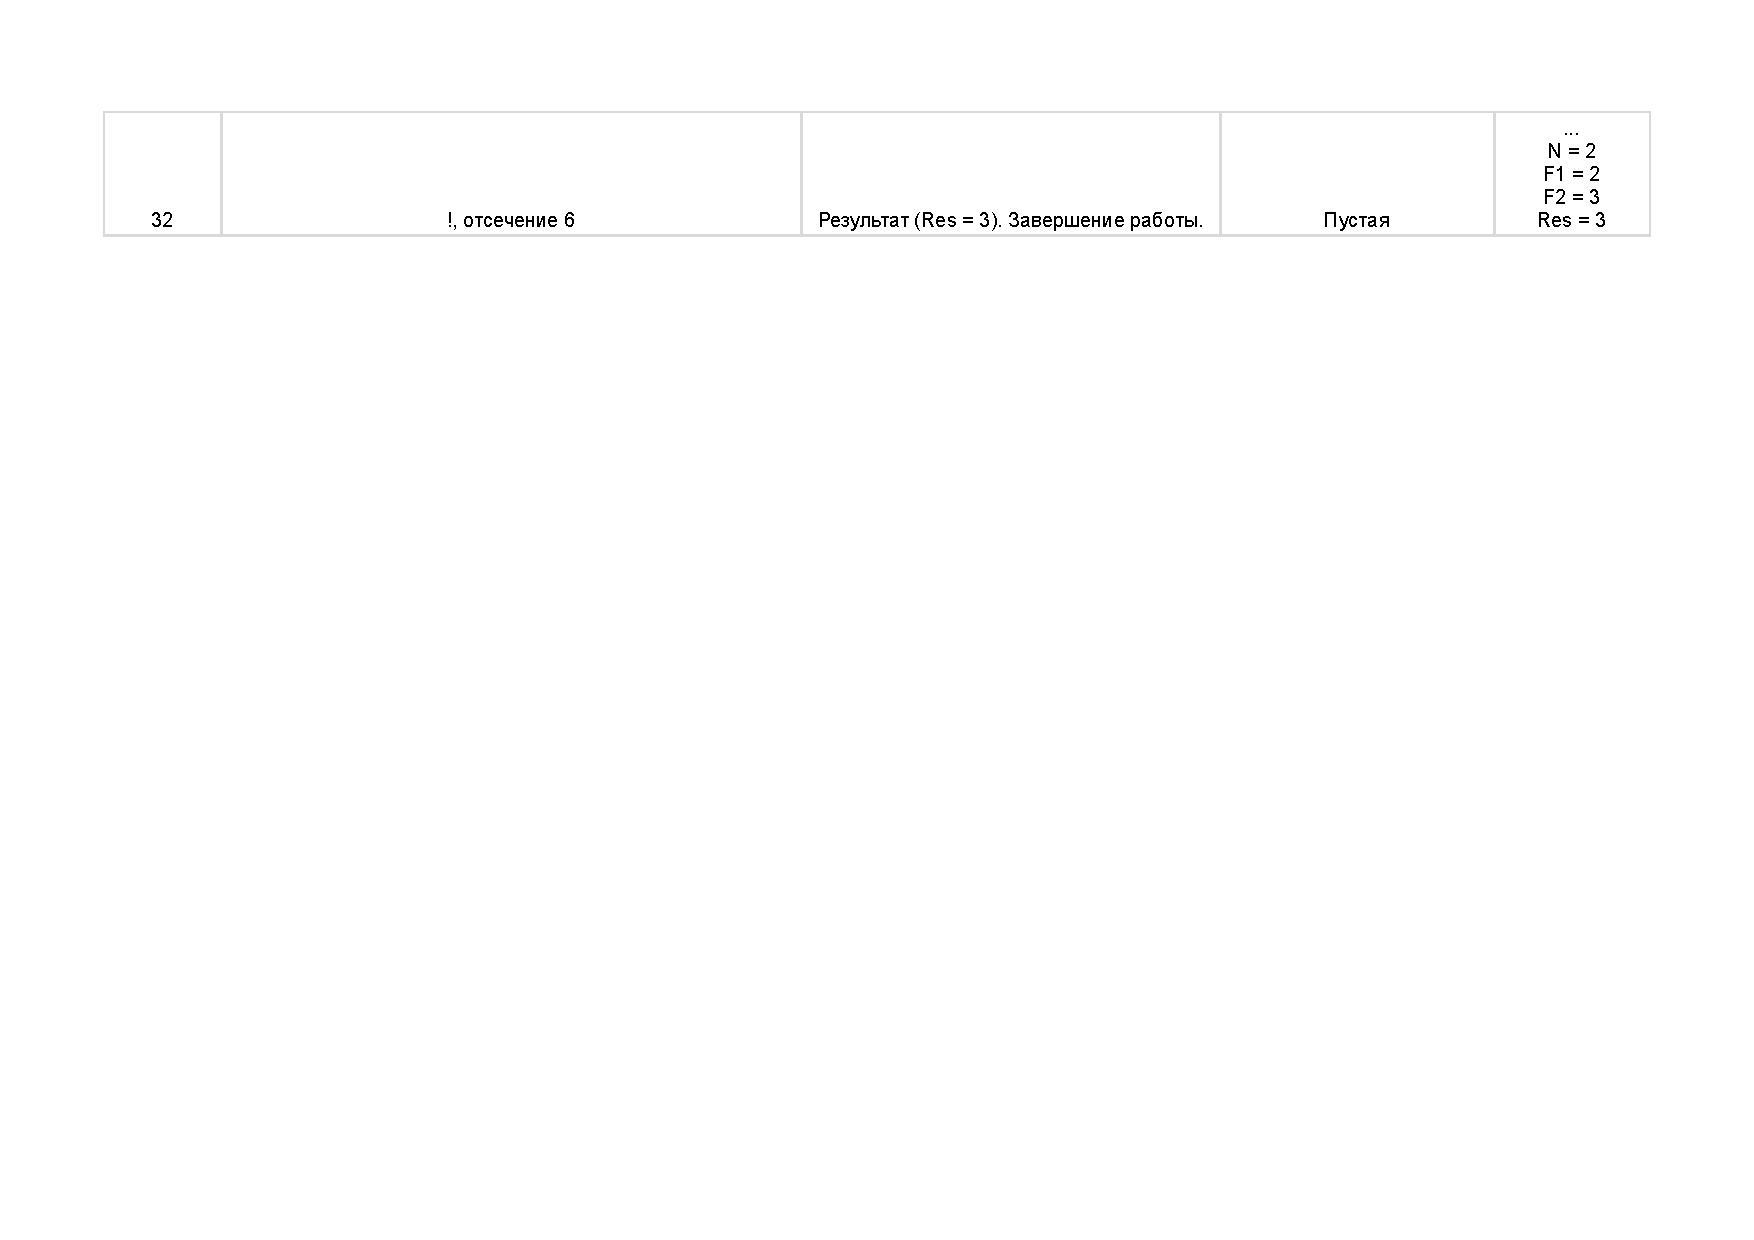
\includegraphics[scale=0.7]{imgs/table_16_02-4.pdf}
	\end{center}
\end{figure}

\end{document}